% begin module improper-integral-comparison-ex9
\begin{frame}
\begin{example} %[Example 9, p. 550]
Show that $\int_0^\infty e^{-x^2}\diff x$ is convergent.
\begin{itemize}
\item<2-> If integral were $\int_{0}^{\infty} e^{-x}\diff x$, we could integrate directly. 
\item<3->  However, the antiderivative of $e^{-x^2}$ isn't an elementary function.
\item<4-| alert@10> Notice that $e^{-x^2} \leq e^{-x}$ for $x\geq 1$.
\item<5-> Now split $\int_0^\infty e^{-x^2}\diff x = \alert<6>{ \int_0^1 e^{-x^2}\diff x} + \int_1^\infty e^{-x^2}\diff x$.
\item<6->  On the RHS, first integral is proper - no affect on convergence.
\end{itemize}
\begin{columns}[c]
\column{.5\textwidth}
\ \uncover<4->{%
\psset{xunit=1.5cm, yunit=1.5cm}
\begin{pspicture}(-0.5,-0.5)(3.2,1.3)
\psframe*[linecolor=white](-0.5,-0.5)(3.200000,1.3)
\tiny
\fcAxesStandard{-0.500000}{-0.5}{3.000000}{1.2}
%Function formula: e^{- x^{2}}
\psplot[linecolor=\fcColorGraph, plotpoints=1000] {0.000000} {3.000000}{2.718281828 x 2.0000000 exp -1.0000000 mul exp }
\rput[t](0.5, 0.45){$y=e^{-x}$}

%Function formula: e^{- x}
\psplot[linecolor=blue, plotpoints=1000] {0.000000}{3.000000}{2.718281828 x -1.0000000 mul exp }
\rput[lb](0.5, 0.9){$y=e^{-x^2}$}

\fcXTickWithLabel{1}{$1$}
\end{pspicture}
%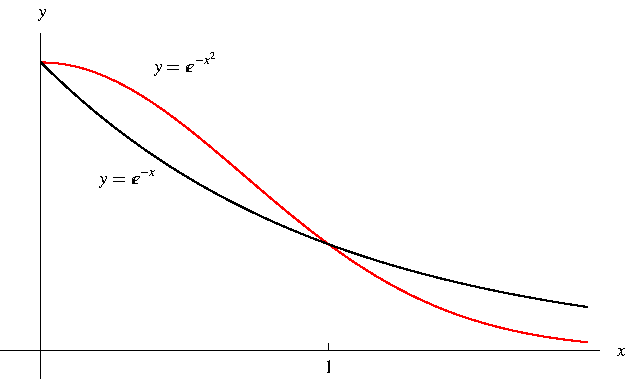
\includegraphics[height=3cm]{improper-integrals/pictures/08-08-ex9.pdf}%
}%
\column{.5\textwidth}
\begin{eqnarray*}
\uncover<7->{%
\alert<handout:0| 10>{\int_1^\infty e^{-x}\diff x}%
}%
& \uncover<7->{ = } & %
\uncover<7->{%
\lim_{t\rightarrow \infty} \int_1^t e^{-x}\diff x%
}\\%
& \uncover<8->{ = } & %
\uncover<8->{%
\lim_{t\rightarrow \infty} \left[ -e^{-x}\right]_1^t
}\\%
& \uncover<9->{ = } & %
\uncover<9->{%
\lim_{t\rightarrow \infty} (e^{-1} - e^{-t})%
}\\%
& \uncover<10->{ = } & %
\uncover<10->{%
\alert<handout:0| 11>{e^{-1}}
}%
\end{eqnarray*}
\end{columns}
\uncover<11->{%
Therefore by the Comparison Theorem, $\int_0^\infty e^{-x^2}\diff x$ converges.
}%
\end{example}
\end{frame}
% end module improper-integral-comparison-ex9
